\newcommand\bytes{128}
\newcommand\digits{9}
\newcommand\base{4}

\section{Introducción}
El propósito de esta estructura de datos llamada \textbf{Integer} es almacenar
un número de un largo inespecificado de dígitos y poder realizar operaciones
aritméticas básicas con el mismo.
\section{Estructura}
A como se puede ver en la Figura~\ref{fig:dig_obj}, la clase \textbf{Integer} es
en esencia una lista enlazada de \textbf{NodeInteger}, cada uno de los cuales
gasta \bytes\ bytes de memoria. Esto en un sistema de x86\_64 equivale a
\the\numexpr\bytes/\base\relax\ \textbf{BasicInteger}, cada uno de estos capaz
de almacenar \digits\ dígitos. Esto implica que un solo \textbf{NodeInteger} por su 
cuenta es capaz de almacenar \digits\ $*$ \the\numexpr\bytes/\base\relax\ dígitos,
lo cual equivale a \the\numexpr\bytes/\base*\digits\relax\ dígitos.
\begin{figure}[H]
\centering
  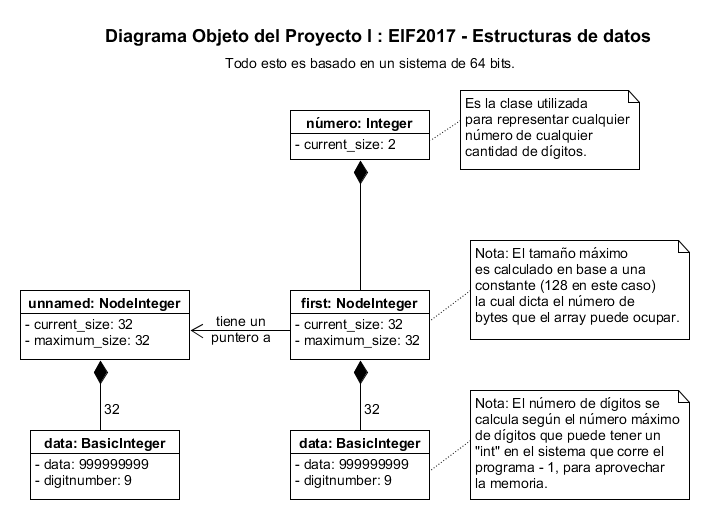
\includegraphics[width=\linewidth]{./img/object_diagram.png}
  \caption{Diagrama objeto de \textbf{Integer}}
\label{fig:dig_obj}
\end{figure}
\section{Desperdicio}
Debido a que cada \textbf{NodeInteger} abarca un total de \bytes\ bytes en esta
implementación el desperdicio de memoria en caso de que un \textbf{NodeInteger}
contenga un 0 se mantiene constante.\\
Tomando $b$ como el tamaño de bytes de cada celda, $b$ equivale a \base\
bytes; y tomando $n$ como el número de celdas de cada \textbf{NodeInteger}, este
equivale a $\frac{\bytes}{b}$; esto implica que la fórmula $d(b, n)$ equivale a
la constante \bytes\ más el número de bytes que un puntero ocupa, el cual
dependiendo de la arquitectura es 4 u 8.\\
En el mejor de los casos, cuando cada uno de los \textbf{NodeInteger} está 
completamente lleno, el desperdicio es 4 y 8 por cada \textbf{NodeInteger} que el
\textbf{Integer} posee. Y en el peor de los casos el desperdicio es $(\bytes\ + 4$
u $8) * IntegerSize$, dependiendo de la arquitectura.
\section{Operaciones aritméticas}
En lo que corresponde a las operaciones aritméticas, se le delegó a las unidades
más básicas, \textbf{BasicInteger} y \textbf{NodeInteger}, las operaciones
básicas de la suma y la resta, debido a la facilidad con la que estas
operaciones se pueden implementar de manera modular. Para las operaciones más
complejas de la multiplicación y la división, estas se implementaron en la clase
\textbf{Integer}.
